\chapter{Evaluation}
For the experiments, Tesla K80 GPU was used, which has 13 SMs and each SM contains 192 SPs. The GPU operates at 562 GHZ with 11.25 GB global memory, 48 KB shared memory/block, 64K registers/block, and 64 KB constant memory. An Intel Xeon Processor E5 family operating at 2.30 GHz was used as a host CPU. The packets were captured using a packet capture file, and there were 100 packets per file. The GPU main function was launched with 260 blocks and 256 threads per block.

\section{Block-Level Parallelism vs. Thread-Level Parallelism}

The total packet processing time was measured by varying the size of the packet. The Rabin-Karp algorithm was used for signature matching. The execution times for thread-level and block-level parallelism are plotted in a log scale shown in Fig. ~\ref{fig:parallelism}. 

\begin{figure}[H]
	\centering
	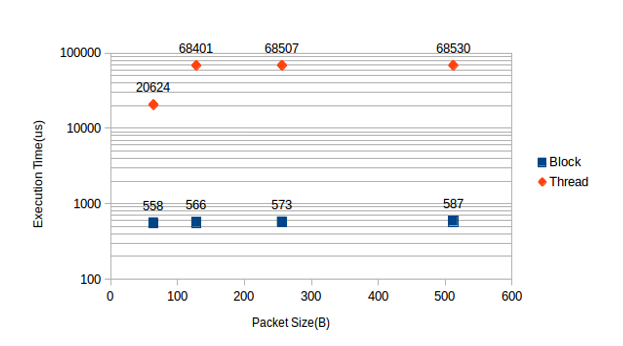
\includegraphics[width=12cm]{parallelism.png}
	\caption{Execution times for packet processing}
	\label{fig:parallelism}
\end{figure}
\squeezeup

As can be seen, the execution time gradually increased with the packet size. Block-level packet processing significantly improved the throughput over thread-level packet processing. This is because of the high level of parallelism that block-level packet processing provides. Note that, block-level processing inspects individual packets with multiple threads. On the other hand, thread-level processing handles one packet per thread. Hence, the individual packet processing time was longer than block-level processing.

\section{Comparison between OpenMP, CPU and GPU solutions}
As shown in Table ~\ref{tab:executionTimes}, the execution times of the Aho-Corasick and the Wu-Manber algorithms were almost stable irrespective of the signature count, while that of the Rabin-Karp algorithm was proportional to the signature count. This is because the Aho-Corasick and the Wu-Manber algorithms are multiple signature-matching algorithms in which the text is searched only once for all the patterns. However, in the Rabin-Karp algorithm, the patterns are searched by iterating over the total number of patterns. 

\begin {table}[H]
\centering
\caption {Execution Times on the GPU} \label{tab:executionTimes}
\begin{tabular}{|c|c|c|c|}
	\midrule
	Number Of Patterns &  Aho-Corasick &  Wu-Manber &  Rabin Karp\\
	\midrule
	10 & 0.222589    & 0.220862 &    26.297111\\
	\midrule
	50 &    0.213149 &    0.212749 &    47.350966\\
	\midrule
	100 &    0.216893 &    0.211166 &    45.577234\\
	\midrule
	200    & 0.217278 &    0.20659    & 59.012978\\
	\midrule
	500    & 0.20355 &    0.206813 &    107.944879\\
	\midrule
	1000 &    0.204189 &    0.240702 & 201.787673\\
	\midrule
	1500 &    0.204285 &    0.225118 &    253.685357\\
	\midrule
	1800 &    0.208605 &    0.204189 &    302.226957\\
	\midrule
\end{tabular}
\end{table}
\squeezeup
The execution times are shown for the optimized version of the algorithms, which were developed using pinned memory. To understand the performance improvement of the GPU-version IDS, I compared the execution times of sequential CPU-based IDS and, parallel CPU-based IDS with OpenMP, and GPU-based IDS with and without pinned-memory optimization. The execution times are listed in Table ~\ref{tab:ahoComparison} and Table ~\ref{tab:wuManberComparison}. 

\begin {table}[H]
\centering
\caption {Performance of Pattern-Matching Algorithms} \label{tab:ahoComparison}
\begin{tabular}{|c|c|c|c|c|}         
	\midrule        
	Number Of Patterns & CPU    & OpenMP &    Not Pinned &    Pinned\\
	\midrule    
	10 &    3005 &    7985 &    0.105183 &    0.222589\\
	\midrule    
	50 &    2973 &    7787 &    0.103743 &    0.213149\\
	\midrule    
	100 &    2781 & 8132 &    0.104735 &    0.216893\\
	\midrule    
	200 &    4420 &    12878 &    0.101759&    0.217278\\
	\midrule    
	500    & 5520 &    23179 &    0.101663 &    0.20355\\
	\midrule    
	1000 &    10185 &    39891 &    0.101151 &    0.204189\\
	\midrule    
	1500 &    7081 &    51755 &    0.103423 &    0.204285\\
	\midrule    
	1800 &    8227 &    68304 &    0.100447 &    0.208605\\
	\midrule
\end{tabular}
\end{table}
\squeezeup
\begin {table}[H]
\centering
\caption {Comparison of Execution Times for the Wu-Manber Algorithm} \label{tab:wuManberComparison}
\begin{tabular}{|c|c|c|c|c|}         
\midrule        
Number Of Patterns & CPU    & OpenMP &    Not Pinned &    Pinned\\
\midrule
10 & 213.698 &    1452.645 &    0.447387 &    0.220862\\
\midrule
50  & 210.193    & 1181.612    & 0.458107    & 0.212749\\
\midrule
100    & 218.394    & 2033.47    & 0.452315    & 0.211166\\
\midrule
200    & 3263.717 &     1231.181 &     0.468123 &     0.20659\\
\midrule
500    &  7188.387 &     1296.764 &     0.454875    & 0.206813\\
\midrule
1000 &     12594.664 &     2411.357 &     0.465852 &     0.240702\\
\midrule
1500 &     18745.097    & 2738.667    & 0.464059 &      0.225118\\
\midrule
1800 &     18564.539    & 1307.96    & 0.452891 &     0.204189\\
\midrule
\end{tabular}
\end{table}
\squeezeup
As can be seen in Fig. ~\ref{fig:speedup}, the GPU-version IDS had 60 times greater speedup than the CPU-version in all three algorithms. Fig. ~\ref{fig:speedup} shows that the speedup increases as the number of patterns increases.  

\begin{figure}[H]
\centering
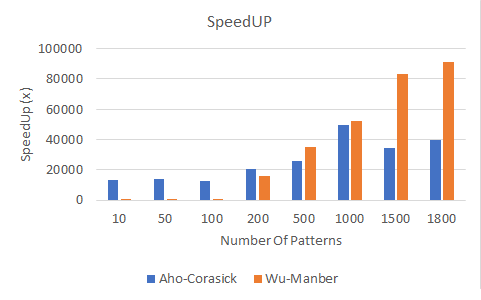
\includegraphics[width=12cm]{speedup.png}
\caption{Speedup of the algorithms on the GPU over the CPU}
\label{fig:speedup}
\end{figure}
\squeezeup
While using the Aho-Corasick algorithm, the OpenMP-based parallel CPU code derived worse performance than sequential CPU code, since the total amount of work done by all threads is larger than the amount of work done by a single thread as explained in the section 5.

In the Wu-Manber algorithm, when the number of patterns is fewer than 200, the sequential CPU code beats the OpenMP version because of the overhead of OpenMP threads. However, when the number of signatures increases, the execution time using OpenMP is significantly shorter than the execution time of sequential version code.

\section{Stall Breakdown}

The evaluation was conducted with 10 packets of 256 bytes and 1800 patterns. Synchronization, memory throttle and execution dependencies had significant differences for pipeline stalls as observed in Fig. ~\ref{fig:issuestallreasons}.

\begin{figure}[H]
	\centering
	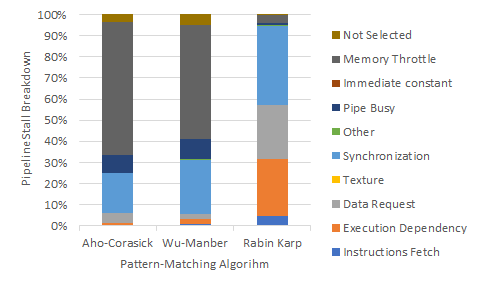
\includegraphics[width=12cm]{issuestallreasons.png}
	\caption{Breakdown for the issue stall reasons}
	\label{fig:issuestallreasons}
\end{figure}
\squeezeup

Memory throttle is caused due to huge number of outstanding memory requests to global memory \cite{bib5}. The global memory load efficiency was < 25\%, and store efficiency was < 15\% due to un-coalesced memory requests to global memory. Un-coalesced memory requests imply the memory requests are outside the 128 or 64 or 32-byte memory gap. The driver coalesces global memory stores and loads of threads of a warp, when all memory accesses are within a 128 or 32 or 64-byte memory segment \cite{bib15}.

Table ~\ref{tab:shift} shows the distribution of pipeline stalls for the three algorithms. In the Aho-Corasick algorithm, the goto function table and the output table are accessed from global memory. Goto table is a two-dimensional array, where the number of rows is same as the number of states and the number of columns is 256. The number of states in the FSM is 447129. Thus, the size of the goto function table is 447129 x 256 x 4 bytes, which equals 447129KB. Due to the huge size of the goto function table, the data could not be saved in shared memory because shared memory size is 16KB. Because the individual threads access the goto table at random positions it leads to un-coalesced memory accesses. 

\begin {table}[H]
\centering
\caption {Pipeline Stall Breakdown} \label{tab:shift}
\begin{tabular}{|c|c|c|c|}
	\midrule
	Issue Stall Reasons &    Aho-Corasick &    Wu-Manber &    Rabin Karp\\
	\midrule
	Instructions Fetch & 0.16\%    & 0.84\%     & 4.74\%\\
	\midrule
	Execution Dependency &    1.27\% &    2.35\% &    26.72\%\\
	\midrule
	Data Request &    4.75\%    & 2.68\% &    25.68\%\\
	\midrule
	Texture     &    0.00\%    & 0.00\%    & 0.00\%\\
	\midrule
	Synchronization &    18.73\%     & 25.44\%    & 37.40\%\\
	\midrule
	Other &    0.20\%    & 0.21\%    & 0.67\%\\
	\midrule
	Pipe Busy &    8.20\%    & 9.45\%    & 0.67\%\\
	\midrule
	Immediate constant    & 0.34\%    & 0.33\%    & 0.00\%\\
	\midrule
	Memory Throttle    & 62.76\%    & 53.82\%    & 3.80\%\\
	\midrule
	Not Selected &    3.60\%    & 4.90\%    & 0.31\%\\
	\midrule
\end{tabular}
\end{table}
\squeezeup

In the Wu-Manber algorithm, the arrays such as shift, prefix size, prefix value, prefix index and pattern are accessed from global memory. The tables are indexed by the hash values, and the hash values calculated by different threads are different. Hence, there would be multiple un-coalesced memory requests to global memory. In the Rabin-Karp algorithm, the memory throttle was much lesser compared to other algorithms. All the threads access the same address of global memory to fetch the pattern hash value. When all the threads in a warp access the same address, the data from global memory are broad-casted to threads in a single memory transaction. 

Synchronization occurs because the threads in a warp are blocked due to the call to the syncthreads function. Before the call to a syncthreads function, a store causes shared store latency. The number of calls to syncthreads are the same across three algorithms.

Thread execution time is the sum of the time a thread spends executing instructions plus the idle time a thread resides waiting for the result from previous instructions. This is due to execution dependency. Multiple threads would share an execution unit of a processor whereby each thread is given a period of time (time slice) to execute before it would be preempted and the execution unit given to another thread. If the threads have un-finished work, it waits for another time slice. The waiting time depends on the number of parallel threads and the availability of resources. In the Aho-Corasick algorithm, the threads perform fewer arithmetic operations on the device (calculations are completed in the  pre-processing stage in the CPU), hence the utilization of execution units was low. In the Wu-Manber algorithm, the hash values are computed for suffixes and prefixes of the text. The hash values are computed using three instructions whereby each instruction is dependent on the result of previous instruction. Hence, the execution dependency was slightly higher than the Aho-Corasick algorithm. In the Rabin-Karp algorithm, each thread computes the hash value for 1076 patterns, and the instruction dependency led to a higher execution dependency when compared to other algorithms.

\section{Resource Utilization}
\vspace{\topsep}
\subsection{Memory Utilization}

Packets are stored in shared memory for the three algorithms. Shared memory load transactions are the number of load requests to shared memory, while shared memory store transactions are the number of store requests to shared memory. The shared memory load transaction count was very high for Rabin-Karp compared to the other two algorithms as shown in Fig. ~\ref{fig:smload}. The reasoning is supported by the shared memory replay overhead shown in Fig. ~\ref{fig:smreplay}.

In the Rabin-Karp algorithm, each thread starts signature matching from its thread index, such that tid 0 accesses the byte in shared memory from index 0, tid 1 from index 1, tid 2 from index 2 and so on. The default 32-bit addressing mode is used in shared memory. The bandwidth of each memory transaction is 32-bits. Even though each thread fetches only 1 byte of data, 4 bytes of data are fetched from shared memory. Since the threads in a warp access the consecutive bytes of the same bank in the shared memory, it led to shared memory bank conflicts.

\begin{figure}[H]
	\centering
	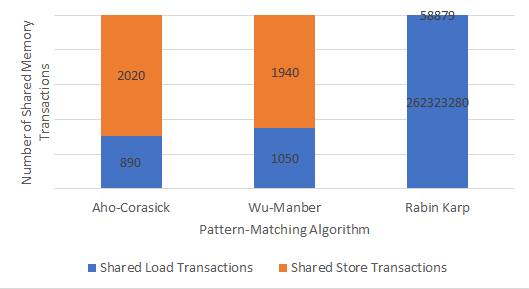
\includegraphics[width=12cm]{smtransactions.png}
	\caption{Shared memory load and store transactions}
	\label{fig:smload}    
\end{figure}
\squeezeup

In the Aho-Corasick and the Wu-Manber algorithms, shared memory replay overhead was approximately equal and very low compared to the Rabin-Karp algorithm. The replay overhead was mainly caused by the DPI on the header in both of these algorithms. Shared memory store was slightly higher in Aho-Corasick algorithm because the values of the next state for the first character of every pattern are stored in shared memory. 

\begin{figure}[H]
	\centering
	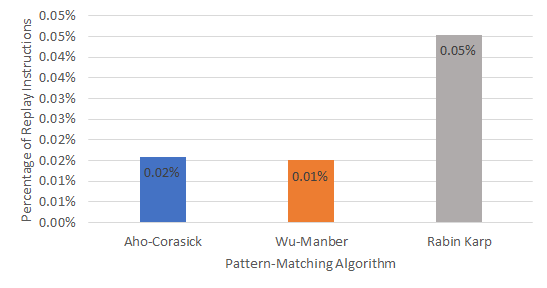
\includegraphics[width=12cm]{smreplay.png}
	\caption{Shared memory replays due to bank conflicts}
	\label{fig:smreplay}
\end{figure}
\squeezeup

Since the number of load or stores are high, shared memory accesses could be replaced by shuffle instructions. Using shuffle instructions, threads in a warp exchange data among themselves without the need of shared memory or global memory. Shuffle instructions have lower latency when compared to shared memory instructions, and do not consume any space.

\subsection{Warp Utilization}

Compute resources are efficiently utilized when all threads in a warp execute the same branch. When this does not happen, the warp execution efficiency is reduced because of the under utilization of the compute resources. During the header check phase of deep packet inspection, only a few threads were active per warp, which led to a decrease in the execution efficiency. The header check phase is common to the three algorithms, and the differences in the graph in Fig. ~\ref{fig:Warp Execution Efficiency} were due to the pattern-matching algorithms.

\begin{figure}[H]
	\centering
	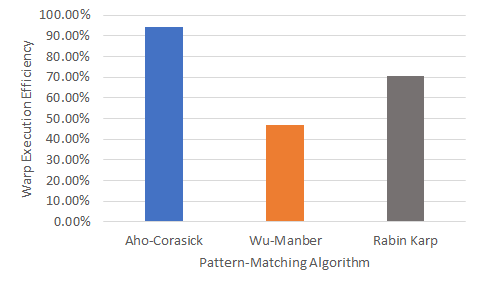
\includegraphics[width=12cm]{warpexecefficiency.png}
	\caption{Average number of active threads executed in a warp}
	\label{fig:Warp Execution Efficiency}    
\end{figure}
\squeezeup

While performing the evaluations, the packets were crafted such that the payload of each packet had the pattern “FICDFICD” repeated multiple times. In the Wu-Manber algorithm, threads which have a shift value as 0 are active in the parallel region as shown in Fig. ~\ref{fig:wumanbranchdiv}. The threads calculate the hash value of the prefixes and iterative over the patterns with the same prefix. When the hash value of the prefix calculated matches the pattern prefix, then the thread becomes active in the parallel region as shown in Fig. ~\ref{fig:wumanbranchdivfor}. The number of threads, which evaluate the above if conditions to be true is low, and it reduces the warp execution efficiency. The pattern “FICDFICD” is repeated throughout the payload of the packet. As two threads out of eight threads have the first condition true, the warp execution throughput for the signature matching is 25\% (8/32).

\begin{figure}[H]
	\centering
	\begin{lstlisting}
	if (shift == 0) {
	\end{lstlisting}
	\caption{Branch divergence in the Wu-Manber algorithm}
	\label{fig:wumanbranchdiv}
\end{figure}
\squeezeup
\begin{figure}[H]
	\centering
	\begin{lstlisting}
	//For every pattern with the same suffix as the text
	for (int i = 0; i < d_PREFIX_size[hash1]; i++) {
	
	//If the prefix of the pattern matches that of the text
	if (hash2 == d_PREFIX_value[hash1 * prefixPitch + i]) {
	\end{lstlisting}
	\caption{Branch divergence in the Wu-Manber algorithm}
	\label{fig:wumanbranchdivfor}
\end{figure}
\squeezeup

In the Aho-Corasick algorithm, there are two conditions which cause branch divergence as shown in Fig. ~\ref{fig:ahocorbranchdiv} and Fig. ~\ref{fig:ahocorbranchdivfor}. If the first character of any pattern exists in the text, the first condition becomes true as shown in Fig. ~\ref{fig:ahocorbranchdiv}. If two characters of the pattern exist in the text, the while loop condition becomes true as shown in Fig. ~\ref{fig:ahocorbranchdivfor}. Since the pattern "FICDFICD" appears in the text, two out of eight threads will have both the conditions true and they execute in the parallel region.

\begin{figure}[H]
	\centering
	\begin{lstlisting}
	if(nextState!=0) {
	\end{lstlisting}
	\caption{Branch divergence in the Aho-Corasick algorithm}
	\label{fig:ahocorbranchdiv}
\end{figure}
\squeezeup
\begin{figure}[H]
\centering
\begin{lstlisting}
while(nextState!=0 && pos<256) {
\end{lstlisting}
\caption{An example while loop that causes branch divergence in the Aho-Corasick algorithm}
\label{fig:ahocorbranchdivfor}
\end{figure}
\squeezeup

Even though the number of threads active per warp for both the Wu-Manber and the Aho-Corasick algorithms are the same, the number of threads that use the execution units is lower for the Wu-Manber algorithm. Since the memory accesses are not coalesced, in the Wu-Manber algorithm, the memory transactions are serialized and the number of threads active per warp are reduced.  In the Rabin-Karp algorithm, the if condition as shown in Fig. \ref{fig:branchdivifrabinkap} is the cause for branch divergence. There are 749 patterns with length \ensuremath{\leq} 64, 1441 patterns with \ensuremath{\leq} 128 and 1743 patterns with length \ensuremath{\leq} 256. Thus, all the threads in warps 3 to 8 will be active. Thread index 54 is the starting thread index for signature matching because the size of the header is 54. Warp 0 is used for checking the validation of the header. The warp efficiency in the Rabin-Karp algorithm is less than the Aho-Corasick algorithm because the percentage of pipeline stalls due to execution dependency is high.

\begin{figure}[H]
	\centering
	\begin{lstlisting}
	if(threadIdx.x <= 256 - patlen) {
	\end{lstlisting}
	\caption{Branch divergence in the Rabin-Karp algorithm}
	\label{fig:branchdivifrabinkap}
\end{figure}
\squeezeup

The number of instructions per warp executed by the Rabin-Karp algorithm is very high, because each thread executes the algorithm for 1786 patterns as shown in Fig. ~\ref{fig:number of instructions per warp}. There are 20 instructions in the algorithm. Thus, total number of instructions executed by the warp is 1,143,040. In the Aho-Corasick and the Wu-Manber algorithms, the algorithm is executed only once for multiple patters and hence, the number of instructions executed per warp are lower.

\begin{figure}[H]
	\centering
	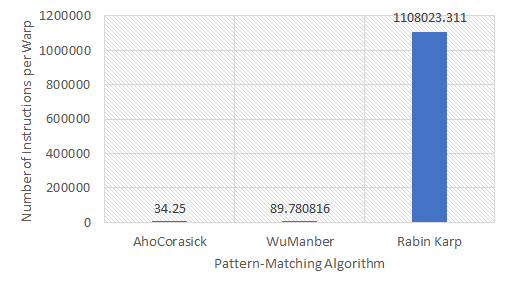
\includegraphics[width=12cm]{instructionsperwarp.png}
	\caption{The number of instructions executed per warp}
	\label{fig:number of instructions per warp}
\end{figure}
\squeezeup


\subsection{SM Utilization}

Fig. ~\ref{fig:smefficiency} shows the average percentage of time each multiprocessor was utilized during the execution of the kernel. An SM is active when there is at least one warp currently executing on the SM. SM utilization is “The percentage of time at least one warp is active on a multiprocessor averaged over all multiprocessors on the GPU.”

\begin{figure}[H]
	\centering
	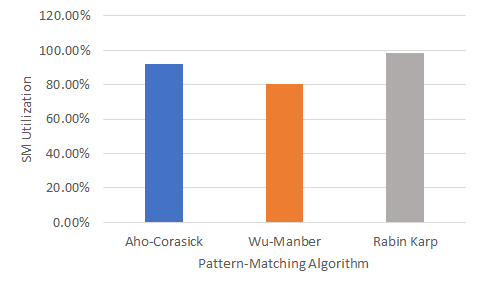
\includegraphics[width=12cm]{smefficiency.png}
	\caption{SM efficiency}
	\label{fig:smefficiency}
\end{figure}
\squeezeup

An SM can become inactive even before the completion of the kernel execution due to three reasons, 1) different execution times of thread blocks, 2) different number of thread blocks scheduled per SM, and 3) combination of the first two reasons.
  
The phenomenon, where some thread blocks are idle and others are active, is known as tail effect. The idle processors can be utilized efficiently by concurrently launching multiple kernels.
In the Wu-Manber and the Aho-Corasick algorithms, the threads will exit early if there is no trace of the pattern in the text. Hence, the thread blocks would have different execution times, and the SM efficiency would be reduced. However, in the evaluation, all the packets are similar and hence, the thread blocks do not have a significant difference in execution times. In the Rabin-Karp algorithm, all threads in warp 3 to 8 are active as explained in the previous section. Thus, the SM efficiency is very close to 100\%. In the Aho-Corasick algorithm and the Wu-Manber algorithm, the warps are active during the search phase. In the Wu-Manber algorithm, different warps get scheduled on the SM to hide the memory latency. Hence, the percentage of time at least one warp is active is reduced.

\section{Cache Hit Rate}

L2 cache was introduced to reduce global memory access bottleneck. The policy used for caching is least recently used (LRU). As L1 cache is disabled by default, it needs to be enabled. In this thesis, only the L2 cache is used. The size of the L2 cache line is fixed at 32 bytes. In Kepler GPU, global memory loads are accessed through the L2 cache (or read-only data cache) \cite{bib5}. In the Rabin-Karp algorithm, cache hit rate is very low because there is no data re-use. However, in the Aho-Corasick and the Wu-Manber algorithms, the tables generated during pre-processing are used often. Hence, the cache hit rate is high as shown in Fig. ~\ref{fig:cachehitrate}.

\begin{figure}[H]
	\centering
	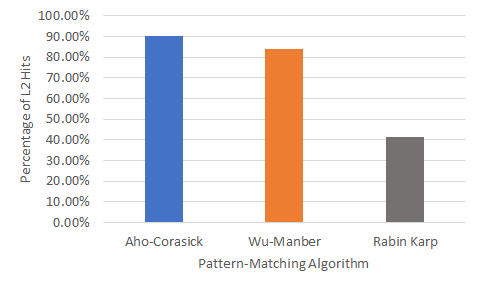
\includegraphics[width=12cm]{cachehitrate.png}
	\caption{L2 hit rate}
	\label{fig:cachehitrate}
\end{figure}
\squeezeup

\section{Pinned Memory Efficiency}
As shown in Fig. ~\ref{fig:pinnedmemoryeffic}, when pinned memory was used, the memory transactions between the CPU and the GPU reduced in the case of the Aho-Corasick and the Wu-Manber algorithms, and the time spent in executing the kernel increased. In the case of the Rabin-Karp algorithm, 98\% of the time was spent in executing the kernel. Thus, there is no significant difference between the graphs.

\begin{figure}[H]
	\centering
	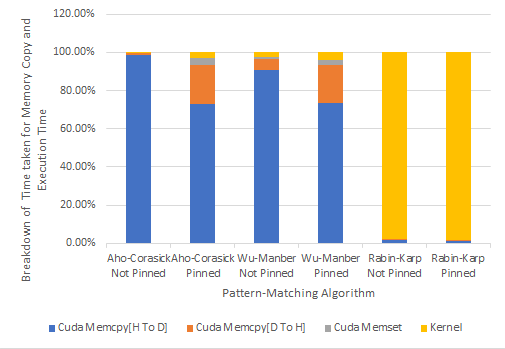
\includegraphics[width=12cm]{pinnedmemoryeffic.png}
	\caption{Pinned memory efficiency}
	\label{fig:pinnedmemoryeffic}
\end{figure}
\squeezeup